%(BEGIN_QUESTION)
% Copyright 2006, Tony R. Kuphaldt, released under the Creative Commons Attribution License (v 1.0)
% This means you may do almost anything with this work of mine, so long as you give me proper credit

Anta at en væske plasseres i en beholder, og at all luft deretter trekkes ut av beholderen med en vakuumpumpe:

$$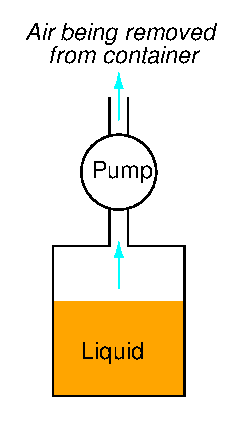
\includegraphics[width=15.5cm]{i00348x01.eps}$$

Beholderen forsegles deretter, og absolutt trykk måles med et trykkinstrument:

$$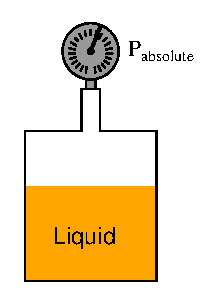
\includegraphics[width=15.5cm]{i00348x02.eps}$$

Når væsken er innestengt i beholderen, vil termisk energi frigjøre noen molekyler til vakuumet over væsken, slik at det dannes damp over væskeoverflaten. Når noen av disse dampmolekylene treffer beholderveggene, kondenserer de tilbake til væske og renner ned i væsken igjen. Når fordampnings- og kondenseringshastigheten blir like, sier vi at væske/damp-prosessen er i \textit{metning}, og trykket inne i beholderen kalles stoffets \textit{mettet damptrykk}. ``Mettet'' betyr ganske enkelt at fordampning og kondensering skjer like raskt, altså at rommet over væsken ikke kan holde flere dampmolekyler.

\vskip 10pt

Anta nå at vi monterer et stempel på beholderen slik at vi kan endre volumet i damprommet:

$$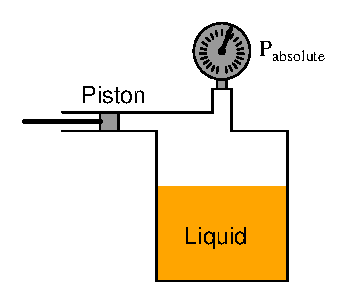
\includegraphics[width=15.5cm]{i00348x03.eps}$$

Hvis systemet når en mettet tilstand (fordampning og kondensering i likevekt), og temperaturen er konstant, hva skjer med trykket i beholderen hvis stempelet beveges innover og volumet dermed reduseres? Øker trykket, minker det, eller forblir det likt?

\vskip 10pt

Anta nå at vi kobler en pumpe til bunnen av denne beholderen slik at vi kan trekke ut noe av væsken uten å slippe inn luft:

$$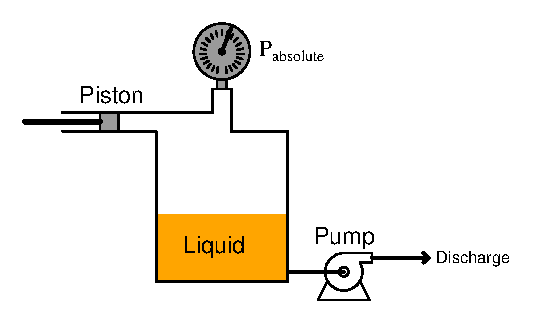
\includegraphics[width=15.5cm]{i00348x04.eps}$$

Hvis systemet når en mettet tilstand (fordampning og kondensering i likevekt), og temperaturen er konstant, hva skjer med trykket i beholderen når væske tappes ut? Øker trykket, minker det, eller forblir det likt?

\underbar{file i00348}
%(END_QUESTION)





%(BEGIN_ANSWER)

I begge tilfeller (stempel inn og væske pumpes ut) blir det først en endring i trykket. Etter at likevekten har etablert seg på nytt, stabiliserer trykket seg imidlertid på nøyaktig samme verdi som før. Mettet damptrykk avhenger ikke av mengden væske eller damp, og heller ikke av volumet i det lukkede rommet.

Til å begynne med vil trykket øke fordi dampen presses inn i et mindre volum (husk $PV = nRT$). Dette øker kondenseringshastigheten (damp til væske) og reduserer fordampningshastigheten (væske til damp). Når overskuddsdamp kondenserer tilbake til væske, synker trykket fordi stoffmengden damp (altså $n$ i $PV = nRT$) blir mindre i rommet over væsken. Til slutt stabiliserer trykket seg på samme verdi som før når systemet igjen er i mettet tilstand.

%(END_ANSWER)





%(BEGIN_NOTES)

%INDEX% Physics, heat and temperature: saturated vapor pressure

%(END_NOTES)
